\subsection[\textless{}T\textgreater]{Templates}

\begin{frame}[fragile]
  \frametitlecpp[17]{Templates}
  \begin{block}{Concept}
    \begin{itemize}
    \item The \cpp way to write reusable code
      \begin{itemize}
        \item like macros, but fully integrated into the type system
      \end{itemize}
    \item Applicable to functions, classes and variables
    \end{itemize}
  \end{block}
  \begin{cppcode}
    template<typename T>
    const T & max(const T &a, const T &b) {
      return a > b ? a : b;
    }
    template<typename T>
    struct Vector {
      int m_len;
      T* m_data;
    };
    template <typename T>
    std::size_t size = sizeof(T);
 \end{cppcode}
\end{frame}

\begin{frame}[fragile]
  \frametitlecpp[98]{Templates}
  \begin{alertblock}{Warning}
    \begin{itemize}
      \item they are compiled for each instantiation
      \item they need to be defined before used
      \begin{itemize}
        \item so all templated code has to be in headers
      \end{itemize}
      \item this may lead to longer compilation times and bigger libraries
    \end{itemize}
  \end{alertblock}
  \newsavebox{\codepiece}
  \begin{lrbox}{\codepiece}
    \begin{minipage}{.35\linewidth}
      \small
      \begin{cppcode*}{gobble=4}
        template<typename T>
        T func(T a) {
          return a;
        }
      \end{cppcode*}
    \end{minipage}
  \end{lrbox}
  \newsavebox{\codepiecea}
  \begin{lrbox}{\codepiecea}
    \begin{minipage}{.4\linewidth}
      \small
      \begin{cppcode*}{gobble=4,linenos=false}
        int func(int a) {
          return a;
        }
      \end{cppcode*}
    \end{minipage}
  \end{lrbox}
  \newsavebox{\codepieceb}
  \begin{lrbox}{\codepieceb}
    \begin{minipage}{.4\linewidth}
      \small
      \begin{cppcode*}{gobble=4,linenos=false}
        double func(double a) {
          return a;
        }
      \end{cppcode*}
    \end{minipage}
  \end{lrbox}
  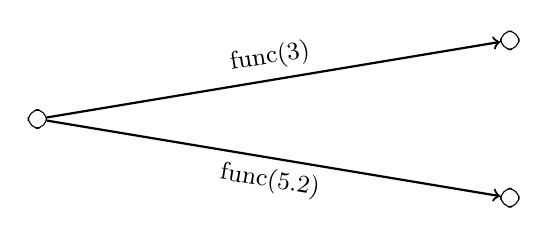
\begin{tikzpicture}[rectangle,rounded corners]
    \draw node (template) [draw] {\usebox{\codepiece}}
          node (templatea) [draw] at (6cm,+1cm) {\usebox{\codepiecea}}
          node (templateb) [draw] at (6cm,-1cm) {\usebox{\codepieceb}};
    \draw[->,thick] (template) -- (templatea) node [above,midway,sloped] {\small func(3)};
    \draw[->,thick] (template) -- (templateb) node [below,midway,sloped] {\small func(5.2)};
  \end{tikzpicture}
\end{frame}

\begin{frame}[fragile]
  \frametitlecpp[98]{Templates}
  \begin{block}{Template parameters}
    \begin{itemize}
    \item can be types, values or other templates
    \item you can have several
    \item default values allowed starting at the last parameter
    \end{itemize}
  \end{block}
  \begin{cppcode*}{}
    template<typename KeyType=int, typename ValueType=KeyType>
    struct Map {
      void set(const KeyType &key, ValueType value);
      ValueType get(const KeyType &key);
    }

    Map<std::string, int> m1;
    Map<float> m2;   // Map<float, float>
    Map<> m3;        // Map<int, int>
  \end{cppcode*}
\end{frame}

\begin{frame}[fragile]
  \frametitlecpp[98]{Templates implementation}
  \begin{cppcode*}{}
    template<typename KeyType=int, typename ValueType=KeyType>
    struct Map {
      // declaration and inline definition
      void set(const KeyType &key, ValueType value) {
        ...
      }
      // just declaration
      ValueType get(const KeyType &key);
    }

    // out-of-line definition
    template<typename KeyType, typename ValueType>
    ValueType Map<KeyType, ValueType>::get
       (const KeyType &key) {
      ...
    }
  \end{cppcode*}
\end{frame}

\begin{frame}[fragile]
  \frametitle{Non-type template parameter \hfill \cpp98 / \cpp17 / \cpp20}
  \begin{block}{template parameters can also be values}
    \begin{itemize}
    \item integral types, pointer, enums in \cpp98
    \item \mintinline{cpp}{auto} in \cpp17
    \item floats and literal types in \cpp20
    \end{itemize}
  \end{block}
  \begin{cppcode*}{}
    template<unsigned int N>
    struct Polygon {
      Polygon(float radius);
      float perimeter() {return 2*N*sin(PI/N)*m_radius;}
      float m_radius;
    };
  \end{cppcode*}
\end{frame}

\begin{frame}[fragile]
  \frametitlecpp[98]{Templates}
  \begin{block}{Specialization}
    templates can be specialized for given values of their parameter
  \end{block}
  \begin{cppcode*}{}
    template<typename F, unsigned int N>
    struct Polygon {
      Polygon(F radius) : m_radius(radius) {}
      F perimeter() {return 2*N*sin(PI/N)*m_radius;}
      F m_radius;
    };

    template<typename F>
    struct Polygon<F, 6> {
      Polygon(F radius) : m_radius(radius) {}
      F perimeter() {return 6*m_radius;}
      F m_radius;
    };
  \end{cppcode*}
\end{frame}

\begin{frame}[fragile]
  \frametitlecpp[17]{Class Template Argument Deduction (CTAD)}
  \begin{block}{CTAD}
    \begin{itemize}
    \item Deduce the template arguments for a class template
    \item Based on construction arguments
    \item Only when no template arguments provided
    \item Since \cpp20: CTAD for aggregates (no constructor needed)
    \end{itemize}
  \end{block}
  \begin{cppcode*}{}
    template<typename A, typename B, typename C = double>
    struct Triple {
      Triple(A a, B b, C c) : a(a), b(b), c(c) {} // C++17
      A a; B b; C c;
    };

    Triple t{42, true, 3.14}; // Triple<int, bool, double>
    Triple<int> t{42, true, 3.14}; // compilation error
    Triple<int, bool> t{42, true, 3.14}; // not CTAD
  \end{cppcode*}
\end{frame}

\begin{frame}[fragile]
  \frametitlecpp[17]{Class Template Argument Deduction (CTAD)}
  \begin{block}{Deduction guides}
    \begin{itemize}
    \item Describe how constructor argument types are mapped to class template arguments
    \end{itemize}
  \end{block}
  \begin{cppcode}
    template<typename A, typename B>
    struct Pair {
     Pair(A a, B b) : a(a), b(b) {}
     A a; B b;
    };
  \end{cppcode}
  \begin{overprint}[\columnwidth]
    \onslide<1>
    \begin{cppcode*}{gobble=2,firstnumber=6}



      Pair p{42, "hello"}; // Pair<int, const char*>
    \end{cppcode*}
    \onslide<2>
    \begin{cppcode*}{gobble=2,firstnumber=6}
      template<typename A>
      Pair(A, const char*) -> Pair<A, std::string>;

      Pair p{42, "hello"}; // Pair<int, std::string>
    \end{cppcode*}
  \end{overprint}
\end{frame}

\begin{frame}[fragile]
  \frametitlecpp[17]{Class Template Argument Deduction (CTAD)}
  \begin{block}{Standard library examples}
    \begin{cppcode*}{}
      std::pair p{1.2, true}; // std::pair<double, bool>
      std::tuple t{1.2, true, 32};
                        // std::tuple<double, bool, int>
      std::vector v{1, 2, 3}; // std::vector<int>
      std::list l{v.begin(), v.end()}; // std::list<int>
      std::array a{1, 2, 3}; // std::array<int, 3>

      std::mutex m;
      std::lock_guard l(m); // std::lock_guard<std::mutex>
    \end{cppcode*}
  \end{block}
\end{frame}

\begin{frame}[fragile]
  \frametitlecpp[98]{The full power of templates}
  \begin{exercise}{Templates}
    \begin{itemize}
    \item go to code/templates
    \item look at the OrderedVector code
    \item compile and run playwithsort.cpp. See the ordering
    \item modify playwithsort.cpp and reuse OrderedVector with Complex
    \item improve OrderedVector to template the ordering
    \item test reverse ordering of strings (from the last letter)
    \item test order based on {\color{blue} \href{https://en.wikipedia.org/wiki/Taxicab_geometry}{Manhattan distance}} with complex type
    \item check the implementation of Complex
    \item try ordering complex of complex
    \end{itemize}
  \end{exercise}
\end{frame}
